\documentclass[english,conference,a4paper]{IEEEtran}

\usepackage[T1]{fontenc}
\usepackage[latin9]{inputenc}
\usepackage{array}
\usepackage{amsmath}
\usepackage{amssymb}
\usepackage{amsthm}
\usepackage{mathdots}
\usepackage{graphicx}
\usepackage{tabularx}
\usepackage{esint}
\usepackage{mhchem}
\usepackage{babel}
\usepackage{textcomp}
\usepackage{algorithm}
\usepackage{algorithmicx}
\usepackage{cite}
\usepackage{bm}
\usepackage{subcaption}
\usepackage{algpseudocode}
%\usepackage{color}
\usepackage[usenames,dvipsnames]{color}

\newcommand{\ignore}[1]{}

\begin{document}

%\title{Overhearing Source Coding in Wireless Multimedia Sensor Networks}
\title{Design and Evaluation of Correlation-Aware Scheduling for Wireless Surveillance Cameras}
\author{
\IEEEauthorblockN{Chang-Yu Song and Hung-Yun Hsieh}
\IEEEauthorblockA{Graduate Institute of Communication Engineering \& \\
Department of Electrical Engineering \\
National Taiwan University, Taipei, Taiwan 106}
%Email: hungyun@ntu.edu.tw}
}

\maketitle

\begin{abstract}
TODO
\end{abstract}

\section{Introduction}
\label{sec:Introduction}
Nowadays, as the concept of Internet of Things (IoT) gradually becomes more and
more important, IP cameras on road can be seen in many countries.
These cameras are connected to the Internet and responsible for some
surveillance applications such as traffic monitoring or crime prevention.
However, the installation of these cameras are often around a small area.
That is to say, image data collected from these cameras might be correlated to
each other.
Therefore, we argue in this paper that we can make use of this correlation and
try to reduce the radio resource used to transmit the image data.

More specifically, if we consider two cameras allocated at a crossroad, we can
analyze their correlation by letting one camera as a I-frame transmitter while
the other as a P-frame transmitter.
Under this assumption, higher correlation level means that we can reduce more
transmission bits when serving the network.
In this paper, we will work on how to serve the wireless multimedia sensor
network (WMSN) better via the overhearing source coding.
We generate the testing images by a 3-D modeling software and these images are
passed through the H.264 reference software to estimate the correlation matrix.
Based on the correlation matrix, we further present a scheduling algorithm to
serve the network so that we can efficiently reduce the total transmission time
needed.

The rest of this paper is organized as follows:
Section~\ref{sec:NetworkScenario} describes our multimedia network scenario and
Scetion~\ref{sec:ProblemFormulation} states our problem formulation.
Section~\ref{sec:SchedulingAlgorithm} solves this problem and
Section~\ref{sec:SimulationResults} shows the simulation results.
Finally, Section~\ref{sec:Conclusion} concludes our work.
%\section{Correlation Analysis and Problem Formulation}
\label{sec::CorrelationAnalysisandProblemFormulation}
In this section, we first details how we analysis the correlation between
cameras in the wireless multimedia sensor network and then formulate our
problem.
\subsection{Correlation Analysis}
\label{sec::CorrelationAnalysis}
As we mentioned before, our purpose in this paper is to reduce the total
transmission time of the wireless multimedia sensor network.
To simplify our problem, we assume that all the cameras in the network need to
transmit its collected image to the aggregator.
Therefore, our problem is to determine the transmission order so that all
cameras in the network can reference from the most correlated frame.

Given a set ${V=\{v_1,v_2, \cdots v_N \}}$ of cameras placed in a city, where
each camera $v_i$ produces image $X_i$.
We now assume that the entropy of independently encoding camera $v_i$ equals
$H(X_{i})$, and	$H(X_{i}|X_{j})$ is the conditional entropy if camera $v_i$
reference from camera $v_j$ when encoding.
Note that if camera $v_i$ tends to reference from camera $v_j$, the
transmission range of camera $v_j$ must cover $v_i$.

To proceed, the correlation between two cameras $v_i$ and $v_j$ can be analyzed
as:
\begin{equation}
\gamma_{ij} = \max \{ 0, 1-\frac{H(X_{i}|X_{j})}{H(X_{i})} \}.
\label{eq::correlationAnalysis}
\end{equation}
The reason why we take the maximum with $0$ is that $H(X_{i}|X_{j})$ can be
larger than $H(X_{i})$ when the scene gathered by camera $v_i$ and $v_j$
differs a lot.
Therefore, in order to make the correlation level always non-negative, we set
${\gamma_{ij}=0}$ when ${H(X_{i}|X_{j})>H(X_{i})}$.
Besides, $\gamma_{ii}$ will not equals to $1$ since there still has some
remaining header in H.264 coding scheme even when using camera $v_i$ to predict
itself.

By analyzing the correlation level between cameras in a network, we can find
the best reference camera for each camera.
That is, if we aim to reduce the transmission time of camera $v_i$, then
choosing camera with the highest ${\gamma_{ij}, \forall j \in V, j \neq i}$
might be a good choice.
However, it rise a problem that we cannot greedy determine the reference camera
by finding the largest value of $\gamma$ for each camera in $V$.
Some of the cameras in $V$ must transmit first so that the later scheduled
P-frame transmitters can reference from them and reduce its transmission time.
Therefore, our goal in this paper is to choose a proper schedule so that the
P-frame transmitter can reference from the most correlated transmitter, and
hence the total transmission time will be reduced.

\subsection{Problem Formulation}
\label{sec::ProblemFormulation}
%\section{Network Scenario}
\label{sec:NetworkScenario}
\begin{figure}
\begin{center}
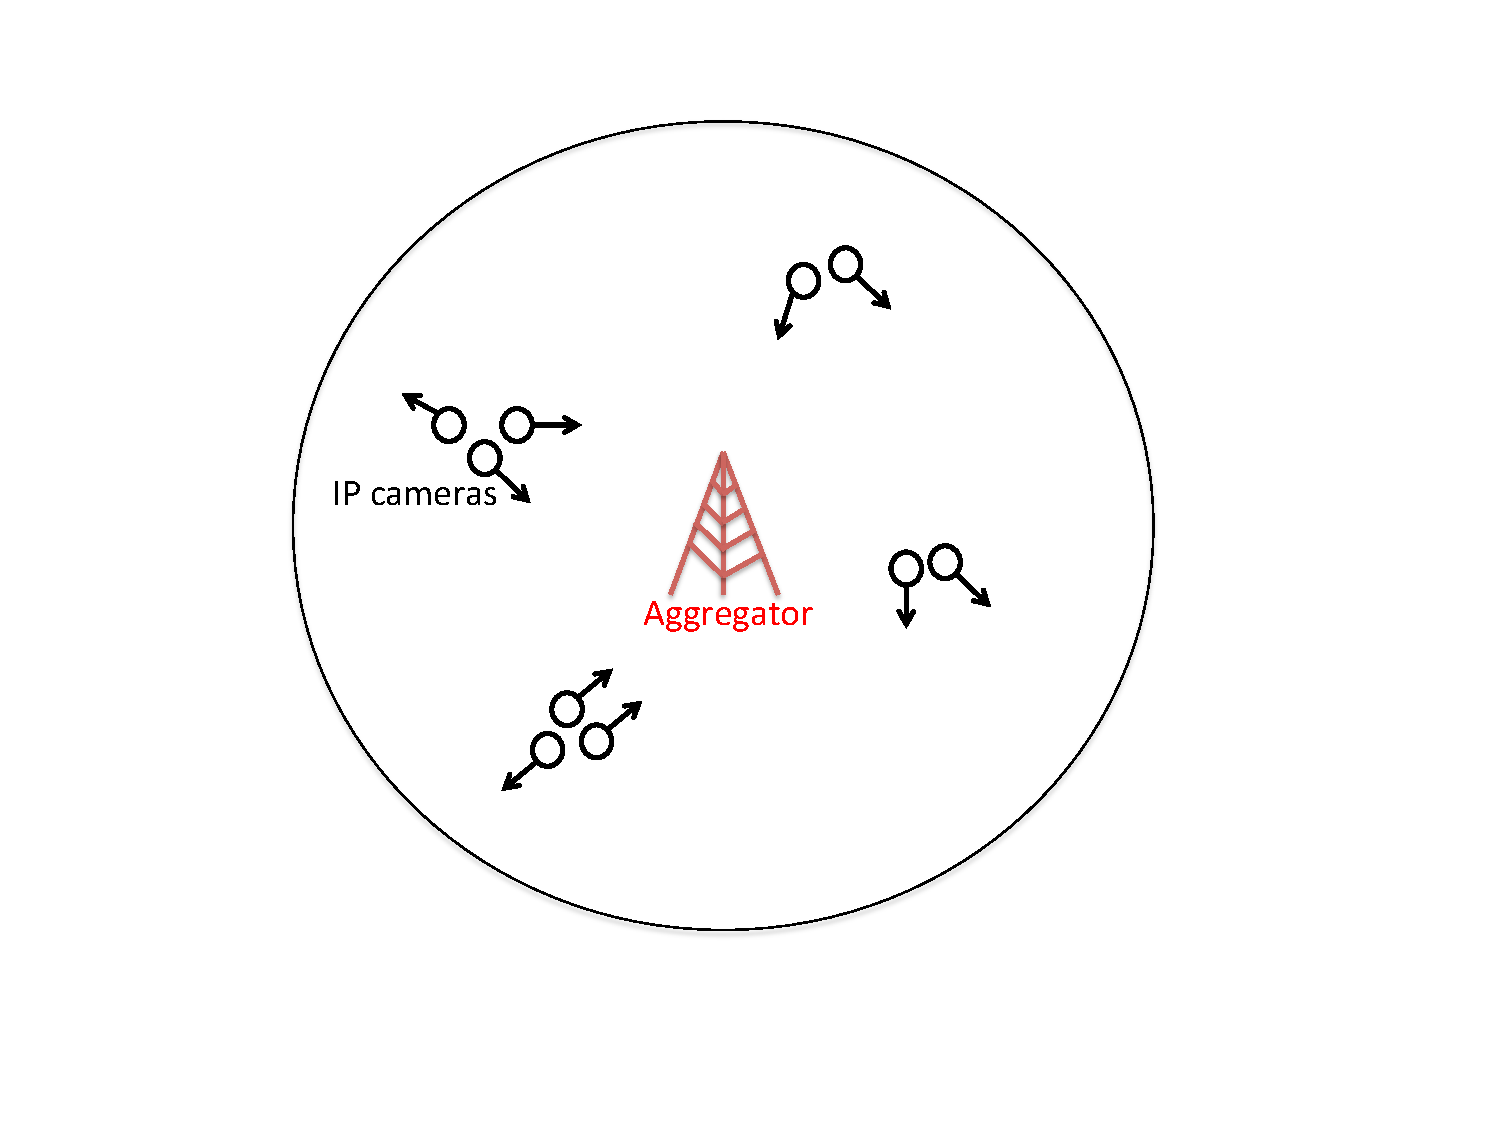
\includegraphics[width=0.7\columnwidth]{surveillanceCamera}
\caption{\label{fig:networkScenario}Network scenario}
\end{center}
\end{figure}
Figure~\ref{fig:networkScenario} shows our scenario for the wireless multimedia
sensor network.
We assume that there is a data aggregator located at the center of a city, which
is responsible for gathering image data collected from all the IP cameras in
this city.
All these images are transmitted through the wireless channel under a TDMA
coding scheme.
Therefore, a camera $i$ can overhear the image data from other cameras if these
cameras are transmitted before $i$ and their transmission range cover $i$.

We now claim that different cameras might have different sensing direction, and
the sensing direction of a given camera is shown by the arrow in
Figure~\ref{fig:networkScenario}.
Besides, several cameras might be grouped together in a small area for a real
world WMSN application.
For example, some companies might install more than one surveillance cameras on
the top of its building so that they can safeguard their
company~\cite{CameraInstallation}.
These cameras is set for sensing different direction; however, the covered range
of these cameras will overlap with each other.
We focus on the overlapping region in this paper since overlapping means
correlation and this correlation can be used for motion prediction in the
image coding.
In this paper, we try to schedule the WMSN for the sake of reducing transmission time for gathering image data.
%%\section{Problem Formulation}

\section{Correlation-based Differential Encoding}
\label{sec::DifferentialEncoding}

\begin{figure}
\begin{center}
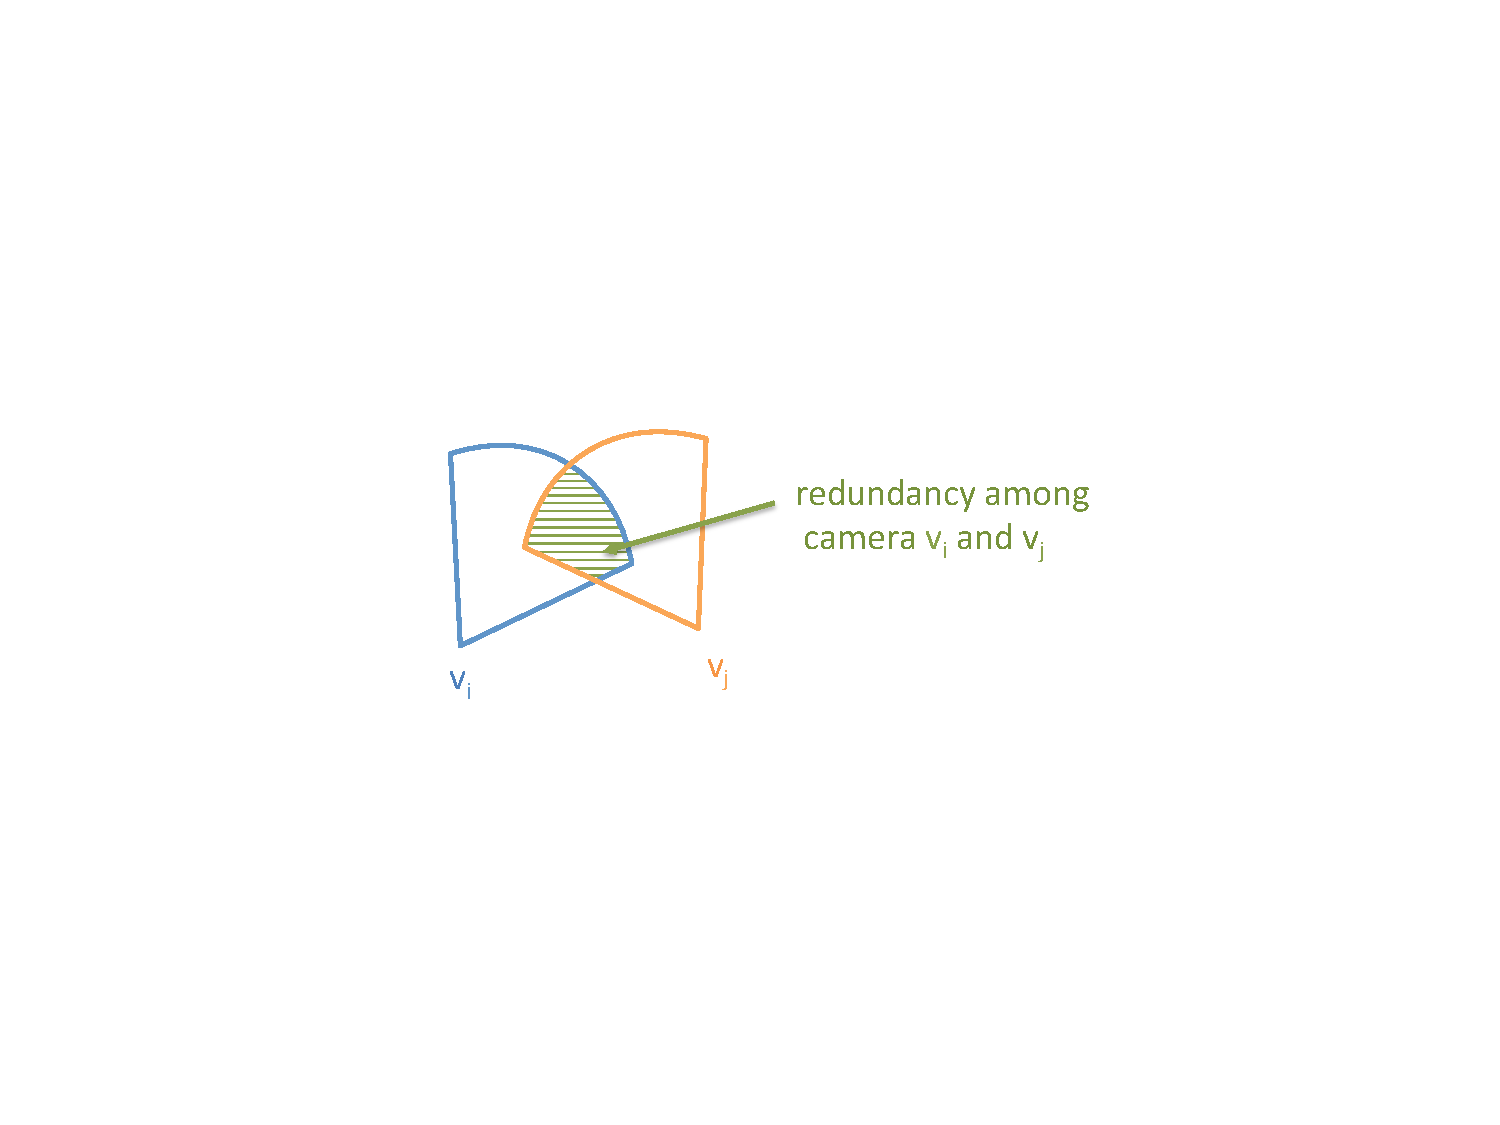
\includegraphics[width=0.7 \columnwidth]{./fig/cameraRedundancy.pdf}
\caption{\label{fig::cameraRedundancy}Redundancy among cameras}
\end{center}
\end{figure}
As we mentioned before, our purpose in this paper is to minimize the total
encoded bits for transmission of a wireless multimedia sensor network.
Given a set ${V=\{v_1,v_2, \cdots v_N \}}$ of cameras placed in a wireless
multimedia sensor network, where each camera $v_i$ produces image $X_i$.
If these cameras are deployed under a dense scenario, there might be some
redundancy among the cameras in $V$.
As Figure~\ref{fig::cameraRedundancy} shows, if two camera $v_i$ and $v_j$ are
installed at a neighboring position and both have the same area of interest,
there might have some overlap among their collected scene.
Therefore, if we serve the network in an independent way (all cameras in $V$
encode its data independently), we might cause a waste of using the limited
radio resource since there is no need to transmit the redundant part.

Since we have mentioned that using a dependent encoding scheme is a more
efficient way to serve the wireless multimedia sensor network.
It rise a problem that how to reduce the transmission of the redundant part.
For the scenario in Figure~\ref{fig::cameraRedundancy}, we can either
compress image $X_i$ based on the prediction of $X_j$ or compress $X_j$ based
on the prediction of $X_i$.
Which mode to choose should depend on the scheduling sequence of cameras, since
a camera can only compress its data based on those previous scheduled cameras.
Therefore, in order to reduce the total required encoded bits of a network, we
will explore an algorithm to determine a proper schedule in the following
sections. 
\section{Related Work}
\label{sec::RelatedWork}
{\color{blue}
Recently, visual sensor networks (VSN) have caught much attention in different
research areas.
One of the most challenging research topics in VSN is the data transmission
issue, which is very different from the conventional scalar sensor
network~\cite{VsnChallenges}.
For example, a surveillance system might have a huge amount of radio resource
demand to provide the image/video transmission over a wireless communication
link.
The authors in~\cite{VehicleSurveillance} motivated the idea of intelligent
vehicle surveillance system for tracking multiple vehicles.
In their model, multiveiw cameras are installed to track vehicles from
different angle of view.
Therefore, in order to operate their system in real-time, there might have some
redundancy among the video transmission and hence motivates us to study how to
reduce the radio resource usage.

One way to exploit the redundancy among multiple surveillance cameras is
through a clustered summary, which is able to browse and search the video in an
efficient way~\cite{ClusteredSynopsis}.
The authors in~\cite{ClusteredSynopsis} argued that regular browsing the
surveillance videos is impossible, since the surveillance videos are often
endless.
Therefore, they improved the browsing efficiency by clustering similar
activities into a shorter video summary.
However, their work focused on the user space efficiency and did not mention
how to collect such huge amount of videos through the wireless communication
links.
In work~\cite{CameraSelection}, the authors reduced the amount of image data
that needs to be transmit over the network by selecting part of the cameras to
report their information.
The selection is based on each cameras' observation and the goal of selection
is to figure out the views that contribute most significantly to the desire
observation.
Our work, on the other hand, required all cameras in the network to transmit
its data while those cameras can reduce their own radio resource usage by
overhearing others' information.
The authors in~\cite{OVVV} and~\cite{VirtualReality} showed the possibility to
use a \emph{Virtual Video} as the test bed of a surveillance systems.
They collected image data from virtual video and used those image for further
investigation.
Therefore, in our work, we also use a $3$D modeling software to generate
quasi-realistic city views and try to reduce the transmission of those views.

Spatial correlation between cameras gives the surveillance networks leverage to
reduce the total amount of encoded bits for transmission.
The authors in~\cite{SpatialCorrelationModel} proposed a spatial correlation
model for cameras deployed in a neighborhood area.
In their model, the correlation of two cameras are determined by their
location and the difference of their sensing direction.
However, the camera views are more complicated so that the correlation cannot
be determined only by its geometric characteristic.
Hence, in order to provide a more realistic model, the work
in~\cite{RealisticModel} gives an investigation of the relation among cameras
through a multiview video coding software.
They analyzed the performance of H.264 multiview video coding of multiple
cameras and showed that the coding cost of two cameras raises as their angular
difference become larger.

One way to deal with the resource reduction problem is through the distributed
video coding~\cite{DVC}, which is based on the Slepian-Wolf's and Wyner-Ziv's
coding theorem.
Distributed video coding is different from the conventional video coding scheme
at both the encoder and decoder.
More specifically, it suggests an encoder encodes individual frames
independently, but the decoder decodes them jointly, which means that the
previous frames are used as a side information at the decoder only.
The authors in~\cite{DVCinMVC} extended the idea of distributed video coding
into multiview systems with spatial correlation among cameras. 
In their work, side information can be generated by exploiting the spatial
correlation and redundancies between different camera's views while the decoder
has the complexity to decode those frames jointly.  
Our work, on the other hand, does not require the decoder to have so much
complexity.
We focus on an overhearing source coding scheme.
That is, each cameras has the possibility to overhear other cameras' frame so
that it can provide inter-frame processing to reduce its encoded bits.

The work in~\cite{MLS} considered overhearing in the wireless multimedia
sensor networks.
They made use of the model proposed in~\cite{SpatialCorrelationModel} and
solved a relaxed integer programming problem to determine a proper schedule for
reducing the most encoded bits.
In this paper, we define a more realistic correlation model and exploit a
\emph{correlation-aware scheduling algorithm} to achieve the same goal as the
optimization problem in~\cite{MLS}.
Simulation result will show that our proposed algorithm can have a better
performance than solving the relaxed optimization problem.
}
\section{Correlation Analysis and Problem Formulation}
\label{sec:CorrelationAnalysisandProblemFormulation}
In this section, we first details how we analysis the correlation between
cameras in the wireless multimedia sensor network and then formulate our
problem.
\subsection{Correlation Analysis}
\label{sec:CorrelationAnalysis}
As we mentioned before, our purpose in this paper is to reduce the total
transmission time of the wireless multimedia sensor network.
To simplify our problem, we assume that all the cameras in the network need to
transmit its collected image to the aggregator and all the cameras can
overhear each other.
Therefore, our problem is to determine the transmission order so that all
cameras in the network can reference from the most correlated frame.

Given a set $V=\{1,2, \cdots N \}$ of cameras placed in a city, we now assume
that the number of transmission bits of camera $i$ equals $H(X_{i})$, and
$H(X_{i}|X_{j})$ is the number of transmission bits when camera $i$ reference
from camera $j$ to provide H.264 coding.
Note that since we assume that all the cameras in the city can hear others'
transmission; therefore, whether camera $j$ is an I-frame transmitter or not
does not influence the value of $H(X_{i}|X_{j})$.
More precisely, if camera $j$ is a P-frame transmitter referenced from camera
$k$, since camera $i$ can gather the data from both $j$ and $k$, it can first
decode the image of camera $j$ and then perform the H.264 encoding.
Hence, we can still obtain the same value of $H(X_{i}|X_{j})$.

To proceed, we now analysis the correlation between two cameras $i$ and $j$ as:
\begin{equation}
c_{ij} = \max \{ (1-\frac{H(X_{i}|X_{j})}{H(X_{i})}),0 \}.
\label{eq:correlationAnalysis}
\end{equation}
The reason why we take the maximum with $0$ is that $H(X_{i}|X_{j})$ can be
larger than $H(X_{i})$ when the scene gathered by camera $i$ and $j$ differs a
lot.
Therefore, in order to make the correlation level always non-negative, we set
${c_{ij}=0}$ when ${H(X_{i}|X_{j})>H(X_{i})}$.
Besides, $c_{ii}$ will not equals to $1$ since there still has some remaining
header in H.264 coding scheme even when using camera $i$ to predict itself. 

\subsection{Problem Formulation}
\label{sec:ProblemFormulation}
The total transmission time needed for the WMSN is highly related to the number
of encoded bits.
That is to say, if we first focus on a camera $i$, we can write the required
transmission time for camera $i$ as:
\[
T_{i} = 
\left\{\begin{tabular}{lp{5.4cm}ll}
\ensuremath{{H(X_{i})}/{C_{i0}}}, &if camera \ensuremath{i} transmits as
an I-frame, \\
\ensuremath{{H(X_{i}|X_{j})}/{C_{i0}}}, &if camera \ensuremath{i} transmits
as an P-frame and reference from camera \ensuremath{j},
\end{tabular}\right.
\]
where $C_{i0}$ is the channel capacity from camera $i$ to the data aggregator.
Therefore, the total transmission time is to sum up all the individual $T_{i}$,
${\forall i \in V}$ written as:
\begin{equation}
T = \sum_{i=1}^{N} T_{i}.
\label{eq:transmissionTime}
\end{equation}

The goal to minimize equation~\eqref{eq:transmissionTime} can be divided into
two sub-problems, including the I-frame selection problem and the P-frame
scheduling problem.
The I-frame selection problem is to choose part of the cameras in the set $V$,
and these selected cameras, say subset $S$, can save the most transmission bits
for the other cameras.
For all the cameras in $V \setminus S$, the P-frame scheduling problem is to
determine which camera to reference with.

\subsection{Dominating Set Problem}
\label{sec::DominatingSet}
{\color{blue}
Recall that our goal in this paper is to determine a proper transmission
schedule.
We here claim that the transmission scheduling problem can be seen as choosing
part of the cameras as {I-frame} transmitters (broadcasters) while the other
cameras are {P-frame} transmitters (listeners).
The transmission schedule is thus simple, we let all the broadcasters to be
transmitted before listeners so that the later scheduled listeners are able to
reference from those previous scheduled broadcasters for reducing its encoded
bits.
Therefore, what we interested in is how to select broadcasters to let those
listeners have the capability to reduce the most encoded bits.
Since the listeners are able to reduce their encoded bits but the broadcasters
cannot, one intuitive idea for radio resource conservation is to select fewest
broadcasters where the transmission range of those broadcasters can cover the
whole network (since a listener can only reduce encoded bits when it can
overhear a broadcaster's transmission).

We now refer to the \emph{Minimum Dominating Set} problem for selecting the
fewest broadcasters in the surveillance network.
In some applications, the \emph{Minimum Dominating Set} problem is formulated
as a integer programming problem~\cite{MDS}.
Therefore, the broadcasters selection problem can be written as:
\begin{align}
\text{minimize} &~~\sum_{i=1}^N \sum_{j=1}^N \alpha_{ii}H(X_j|X_i),\nonumber \\
\text{subject to} &~~A \vec{\alpha} \succeq k \vec{1}, \nonumber \\
 &~~\alpha_{ii} \in \{ 0,1 \},
\label{eq::MDS}
\end{align}
where $A$ is an adjacency matrix indicates the overhearing capability ($i-j$
entry $=1$ if camera $v_i$ is able to overhear camera $v_j$) and $\vec{\alpha}$
is a vector where its $i^{th}$ component is $\alpha_{ii}$.
The ides of Problem~\eqref{eq::MDS} is that we want to select a subset of
broadcasters so that they can have the minimum encoded bits if other listeners
reference from those broadcasters.
The first constraint of Problem~\eqref{eq::MDS} is to protect that all cameras
can have at least $k$ candidate reference broadcasters (covered by the
transmission range of at least $k$ broadcasters).
By relaxing the second constraint of Problem~\eqref{eq::MDS} from ${\alpha_{ii} 
\in \{0,1\}}$ to ${0 \leq \alpha_{ii} \leq 1}$, we can get a linear programming
problem as:
\begin{align}
\text{minimize} &~~\sum_{i=1}^N \sum_{j=1}^N \alpha_{ii}H(X_j|X_i),\nonumber \\
\text{subject to} &~~A \vec{\alpha} \succeq k \vec{1}, \nonumber \\
 &~~0 \leq \alpha_{ii} \leq 1,
\label{eq::relaxedMDS}
\end{align}
Therefore, Problem~\eqref{eq::relaxedMDS} can be solved easily as a
conventional linear programming problem.
After obtaining the value of $\vec{\alpha}$, camera $v_i$ is selected as a
broadcaster with probability $\alpha_{ii}$ and the rest listeners will choose
the best broadcasters as its reference camera.

Note that $k=1$ in the conventional \emph{Minimum Dominating Set} problem since
the goal of \emph{Minimum Dominating Set} problem is to select the fewest nodes
to cover the whole graph.
However, $k=1$ is not suitable in our paper because if a camera $v_i$ can only
select its reference frame from one candidate broadcaster, it happens that the
broadcaster is not correlated with camera $v_i$, causing that the system
performance becomes lower. 
Therefore, we here give the motivation to increase the value of $k$ in
Problem~\eqref{eq::relaxedMDS} and the influence of $k$ will be shown in our
evaluation results.

}
{\color{OliveGreen}
%We also try use a greedy algorithm to solve the broadcaster selection problem
%in a surveillance cameras network.
%First, we need to mention that any maximal independent set (MIS) is a
%dominating set if they consider the same graph, and constructing a MIS can be
%done by a greedy algorithm~\cite{MISisDS}.
%In reference~\cite{MIS}, the authors generate the MIS by an adaptive greedy
%function.
%In this paper, we refer to the idea in~\cite{MIS} but slightly change the
%greedy objective
We also try to use graph theory to solve the broadcaster selection problem in
surveillance cameras network.
Note that the idea of $k$ introduced in Problem~\eqref{eq::relaxedMDS} is
similar to the $k$-tuple dominating set problem.
The authors in~\cite{ICGA} proposed an \emph{ICGA} algorithm which is able to
generate a $k$-tuple dominating set based on centralized decision.
The \emph{ICGA} algorithm constructs a dominating set first and iteratively add
node whose dominator neighbors is less than $k$ into the dominating set by a
greedy criteria.
We here first construct a dominating set $\mathcal{D}$ by the algorithm
proposed in~\cite{MIS}, and apply the \emph{ICGA} algorithm for generating the
$k$-tuple dominating set $\mathcal{D}_k$.
The overall procedure of the algorithm is summarized in
Algorithm~\ref{alg::kTupleDS}, and the performance will also be compared in
our evaluation results.

}

\begin{algorithm}[t]
\caption{Constructing a $k$-tuple dominating set $\mathcal{D}_k$
\label{alg::kTupleDS}}
\begin{algorithmic}[1]
\State Construct a dominating set $\mathcal{D}$ using GRASP~\cite{MIS}
\State $\mathcal{D}_k \gets \mathcal{D}$
\While{There has a node whose number of dominator neighbors is less than $k$}
\State $\mathcal{F} \gets$ All the nodes whose number of dominator neighbors is
less than $k$
\State Add the node that dominates the largest number of nodes in $\mathcal{F}$
to $\mathcal{D}$ 
\State $\mathcal{D}_k \gets \mathcal{D}$ 
\EndWhile
\end{algorithmic}
\end{algorithm} 
\subsection{Scheduling Algorithm}
\label{sec::SchedulingAlgorithm}

%In this section, we show how we determine a proper schedule for minimizing the
%total encoded bits required for a wireless multimedia sensor network.
%On one hand, for a camera $v_i$, if we schedule it at a former position, there
%will be more cameras that can be benefited by overhearing $v_i$'s transmission.
%On the other hand, if $v_i$ is scheduled later, it will have more candidate
%cameras to select as its reference frame, and hence $v_i$ can have a greater
%opportunity to reduce more encoded bits.

To schedule the given set of cameras for minimizing the total encoded bits,
%note that the trade-off involved in determining the scheduling order of any
%camera is the amount of bits that can help others save and the amount of bits
%that it can save by overhearing
%we first explore the trade-off
%between putting a camera at a former or later position.
denote $\Phi \subset V$ as the subset of cameras already scheduled and
%an already scheduled cameras sequence $\Phi \subset V$, we can
$\phi_l$ as the last scheduled camera in $\Phi$.
Now consider two different schedules:
%In equation~\eqref{eq::resourceDifference}, we observe two different schedule,
\emph{Schedule $1$}: ${\phi_l \leftarrow v_i \leftarrow v_j}$ ($v_i$ is scheduled
immediately after $\phi_l$) and
\emph{Schedule $2$}: ${\phi_l \leftarrow v_j \leftarrow v_i}$ ($v_j$ is scheduled
before $v_i$).
%, and we try to calculate the difference of their encoded bits.
%The first two terms in equation~\eqref{eq::resourceDifference} are under camera
%$v_i$'s perspective while the last two terms are for camera $v_j$.
If the transmission order is changed from \emph{Schedule $1$} to \emph{Schedule
$2$}, the reference frame of camera $v_i$ will change from $\phi_l$ to $v_j$,
resulting in a change in the amount of encoded bits for camera $v_i$
%a resource difference of camera $v_i$
as ${H(X_i|X_{\phi_l}) - H(X_i|X_j)}$.
For camera $v_j$, the difference in the amount of encoded bits is
%In this case, For the same reason, the resource difference of camera $v_j$ is
${H(X_j|X_i)-H(X_j|X_{\phi_l})}$.
%
Therefore, the total amount of change in the amount of encoded bits by changing
from {\em Schedule $1$} to {\em Schedule $2$} is:
%resource difference of two cameras $v_i$ and $v_j$ as:
\begin{align}
\Delta R(v_i,v_j) &=  \{ H(X_i|X_{\phi_l})-H(X_i|X_j) \} \nonumber \\
			      &+  \{ H(X_j|X_i)-H(X_j|X_{\phi_l}) \}.
\label{eq::resourceDifference}
\end{align}
%where $\phi_l$ is the last scheduled camera in $\Phi$.
%
Clearly,
%An interpretation of equation~\eqref{eq::resourceDifference} is that
if the amount of encoded bits can be reduced by changing
%the scheduled position of two adjacent cameras $v_i$ and $v_j$
from \emph{Schedule $1$} to \emph{Schedule $2$}, then camera $v_i$ should
be scheduled after camera $v_j$.

Based on this concept, let $v_i$ and $v_j$ be two different unscheduled cameras.
$\Delta R(v_i,v_j)$ as defined in Equation~\eqref{eq::resourceDifference} is the
difference in the amount of encoded bits if camera $v_i$ is not the first camera
to schedule after $\phi_l$
%scheduled right after $\Phi$
but deferred to the next scheduling position after camera $v_j$.
%
The proposed scheduling metric for each unscheduled camera $v_i$ can be written as:
\begin{equation}
\omega_i = \max_{v_j \in \Phi^c, v_j \neq v_i} \Delta R(v_i,v_j),
\label{eq::schedulingMetric}
\end{equation}
%
where $\Phi^c = V \setminus \Phi$ is the subset of all unscheduled cameras.
%
The proposed scheduling algorithm thus is to choose camera
\begin{equation}
v_k = \underset{v_i \in \Phi^c}{\arg\min}~\omega_i
\label{eq::scheduledCamera}
\end{equation}
%
as the next camera to be scheduled 
%, where camera $v_k$ is a camera that can potentially 
for reducing the largest amount of encoded bits.
% if it is scheduled right after $\phi_l$.
As  Algorithm~\ref{alg::schedulingAlgorithm} shows,
the algorithm starts with $\Phi = \emptyset$ and iteratively chooses a camera
to schedule based on Equation~\eqref{eq::scheduledCamera}.
%We now summarize our proposed scheduling method as follows:
%
%Algorithm~\ref{alg::schedulingAlgorithm} shows the proposed algorithm
%for determining the scheduling orders of the given set of cameras.
%Based on the above discussion, we now give the idea of our scheduling
%algorithm in WMSN.


\begin{algorithm}[t]
%\caption{Solving problem~\eqref{eq::objective} based on scheduling metric}
\caption{Proposed scheduling algorithm\label{alg::schedulingAlgorithm}}
\begin{algorithmic}[1]
\State $\Phi \gets \emptyset$, $\Phi^c \gets V$
\While{$\Phi^c \neq \emptyset$} //loop until all cameras have been scheduled
\State $\omega_i \gets \underset{v_j \neq v_i, v_j \in \Phi^c}{\max} \Delta R(v_i,v_j),
\forall v_i \in \Phi^c$ //calculate the scheduling metric for all unscheduled
cameras
\State $v_k \gets \underset{v_i \in \Phi^c}{\arg\min}~\omega_i$ //choose camera
with the smallest scheduling metric as the next
\State $\Phi \gets \Phi \cup \{ v_k \}$ //record $v_k$ as a scheduled camera
\State $\Phi^c \gets \Phi^c \setminus \{ v_k \}$ //remove $v_k$ from the
unscheduled cameras set
\State $\phi_l \gets v_k$ //update the last scheduled camera in $\Phi$
\EndWhile
\end{algorithmic}
\end{algorithm} 

\section{Performance Evaluation} %Overhearing Experiments}
\label{sec::OverhearingExperiments}
%


%In this section, we first describe the experiment settings and then show the
%our simulation settings about how we
%generate the testing images and then give some discussions about the experiment
%evaluation results for the algorithm proposed in Section~\ref{sec::SchedulingAlgorithm}.

\subsection{Experiment Settings}
\label{sec::ExperimentSettings}

To create quasi-realistic $3$D city views, we make use of an open-source
%To show the advantage of overhearing source coding in the wireless multimedia
%sensor network under a more realistic scenario, we make use of an open source
$3$D modeling software~\cite{Blender} and a $3$D city generator~\cite{Suicidator}.
%called suicidator~\cite{Suicidator}.
%Create detailed city backgrounds
%Blender is a powerful $3$D modeling software that we can use it to generate
%$3$D objects.
%We can use a python script to control the position of all these $3$D objects in
%Blender as well as the lighting source.
%Therefore, we can create a more realistic city scene and make our experiment
%more practical.
%Besides, we also use a free
%A Blender addon called suicidator~\cite{Suicidator} is also used
%to generate a $3$D city for installing camera at crossroads.
%The free version of suicidator can generate a city with size $500 m^2$.
%By setting different parameters in suicidator, we can create a different city
%view.
%For example, we can change the density of streets so that the city looks more
%crowded, and we can also change the texture of buildings to make the city
%different.
A total of $30$ cameras are then deployed at different locations (crossroads)
inside the city of size $500 m^2$ (limited by the capacity of the modeling software)
%After creating these objects, Blender allows us to install cameras at a target
%position and a fixed sensing direction for collecting testing images.
for collecting the desired city snapshots (${1280 \times 720}$ HD images).
Then, H.264~\cite{JMVC} is used to encode the images
collected by individual cameras with or without reference frames.
% to analysis the correlation
%
%Besides, we also use a free Blender addon called suicidator~\cite{Suicidator}
%to generate a $3$D city for installing camera at crossroads.
%The free version of suicidator can generate a city with size $500 m^2$.
%By setting different parameters in suicidator, we can create a different city
%view.
%For example, we can change the density of streets so that the city looks more
%crowded, and we can also change the texture of buildings to make the city
%different.
%Therefore, by using Blender and suicidator, we can collect various scenes to
%verify our proposed algorithm under a more realistic scenario.
%The steps of our experiment settings is summarized as follows:
%\begin{enumerate}
%\item Create a $3$D city in Blender using the suicidator addon.
%\item Install $30$ cameras at different crossroads of the $3$D city.
%\item Collect images from those cameras.
%\item Use a H.264 reference software~\cite{JMVC} to analysis the correlation
%between cameras.
%\end{enumerate}
%
Figure~\ref{fig::cityAndCamera} shows the $3$D city view and the deployment
locations for $30$ cameras.
%our camera deployment in Blender.
With reference to real-world applications,
%~\cite{CameraInstallation}, multiple
multiple cameras are deployments at one crossroad for capturing views from different angles.
The arrow in Figure~\ref{fig::cameraDeployment} is the sensing direction of
each camera while different groups of cameras are shown by different colors.
%(purple color are used for cameras which has not been grouped with other
%cameras).
%Note that we might install more than one camera at a crossroad since some of
%the real-world WMSN applications do so~\cite{CameraInstallation}.
%Each camera is responsible for collecting images for their own area of
%interest (determine by its position and sensing direction).
%To proceed, we now show how we install cameras at a given crossroad.
\ignore{
Figure~\ref{fig::crossroadCamera} gives one group of $3$ cameras deployed at one
crossroad, and
%Suppose at some of the crossroads in the city, we install $3$ cameras and each
%camera has its own sensing direction, the position of cameras is similar to the
%deployment shown in Figure~\ref{fig::crossroadCamera}.
%Obviously, the scenes of these $3$ cameras at the same crossroad is correlated
%with each other since there exists some overlap of their area of interest.
Figure~\ref{fig::testImages} shows the collected images of the $3$ cameras.
%camera deployment of Figure~\ref{fig::crossroadCamera}.
%
It can be observed that images collected by different cameras are highly correlated,
especially for those at the same crossroad, due to the overlap in the view angles.
%We can see in Figure~\ref{fig::testImages} that there exists some similarity
%between collected images at the same crossroad.
%Therefore, the total encoded bits can be reduced if we make use of this
%correlation in a proper way.
}
{\color{blue}

Based on the above settings, we can obtain the amount of encoded bits
(${H(X_1), H(X_2), \cdots H(X_{30})}$) of each camera by independent encoding
its snapshot (${X_1, X_2, \cdots X_{30}}$) through the H.264 reference
software.
The correlation between two cameras (${H(X_i|X_j),i\neq j,1\leq i,j\leq 30}$)
is then analyzed by the multiview encoding of two different snapshots.
Therefore, we can generate a correlation matrix $\mathcal{H}$ where the $i-j$
entry of $\mathcal{H}$ is $H(X_i|X_j)$.
The correlation matrix $\mathcal{H}$ can be further used for our scheduling
algorithm described in Section~\ref{sec::SchedulingAlgorithm}.
}

\begin{figure}[t]
\begin{center}
\begin{subfigure}[b]{0.9\columnwidth}
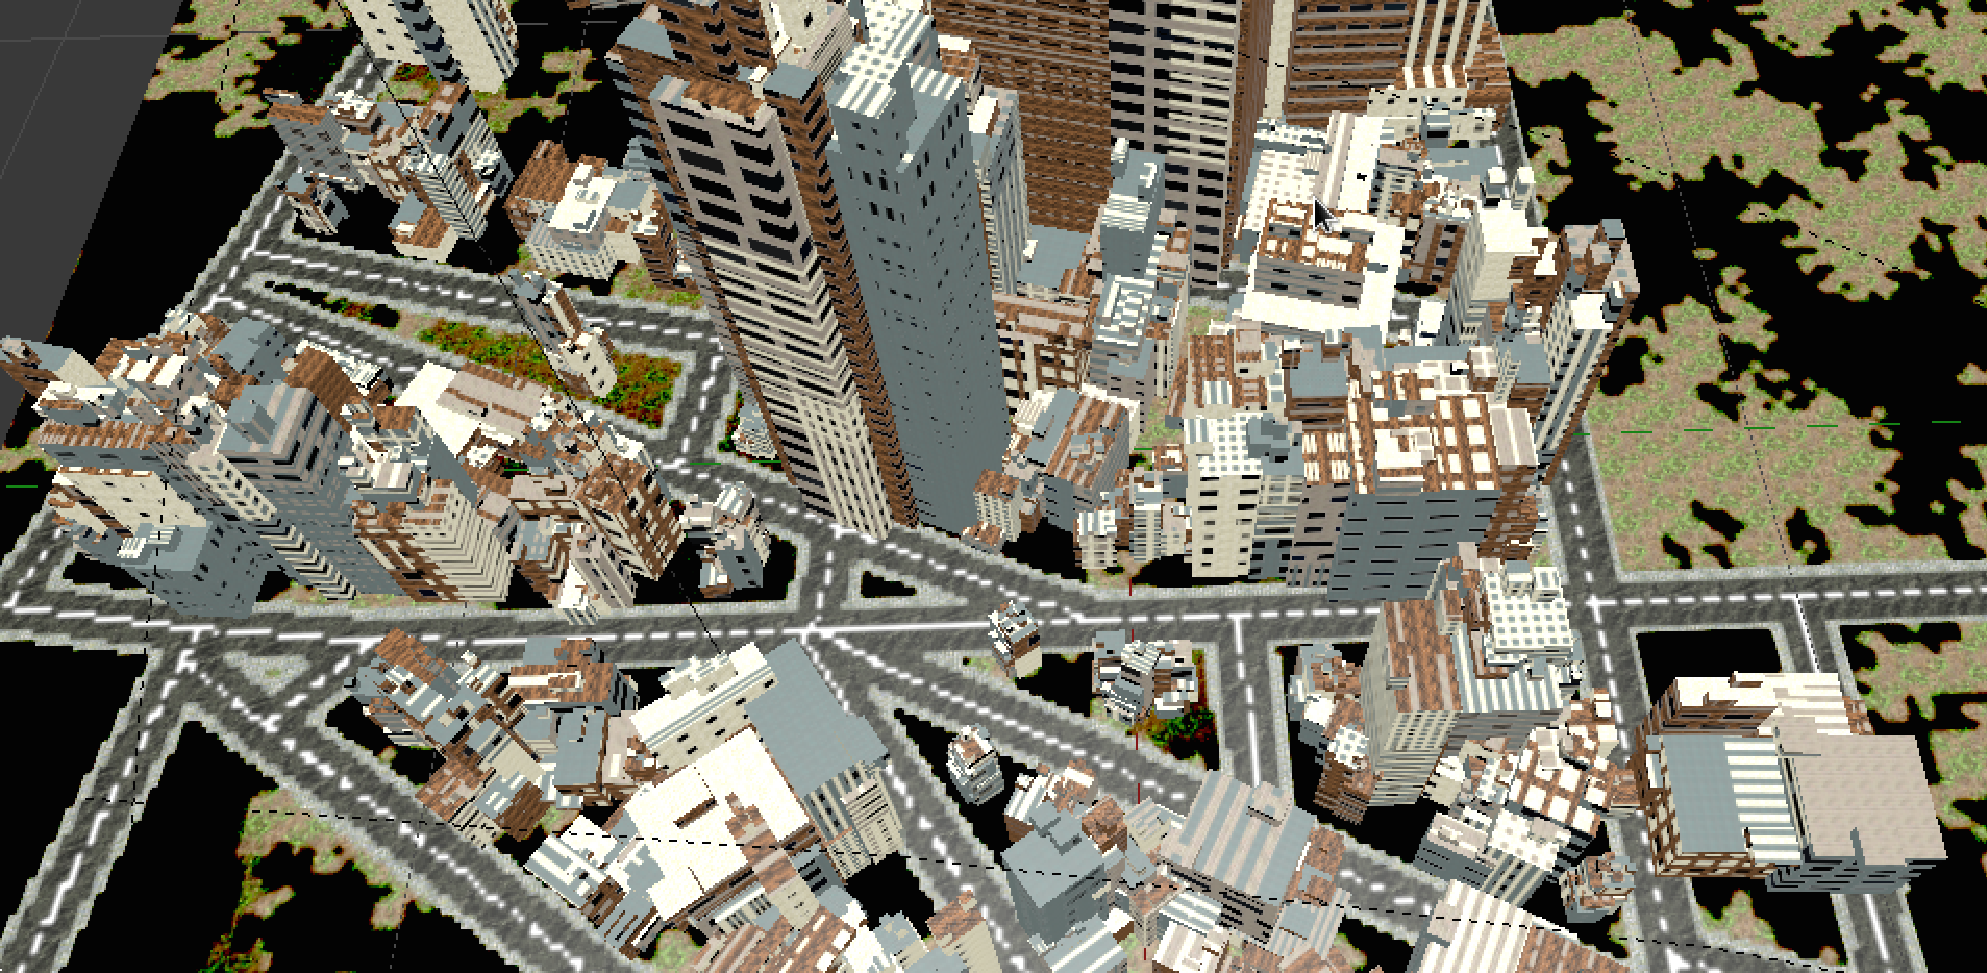
\includegraphics[width=0.9\columnwidth]{./fig/cityView.pdf}
\caption{\label{fig::cityView}City view}
\end{subfigure}
\hfill
\begin{subfigure}[b]{0.9\columnwidth}
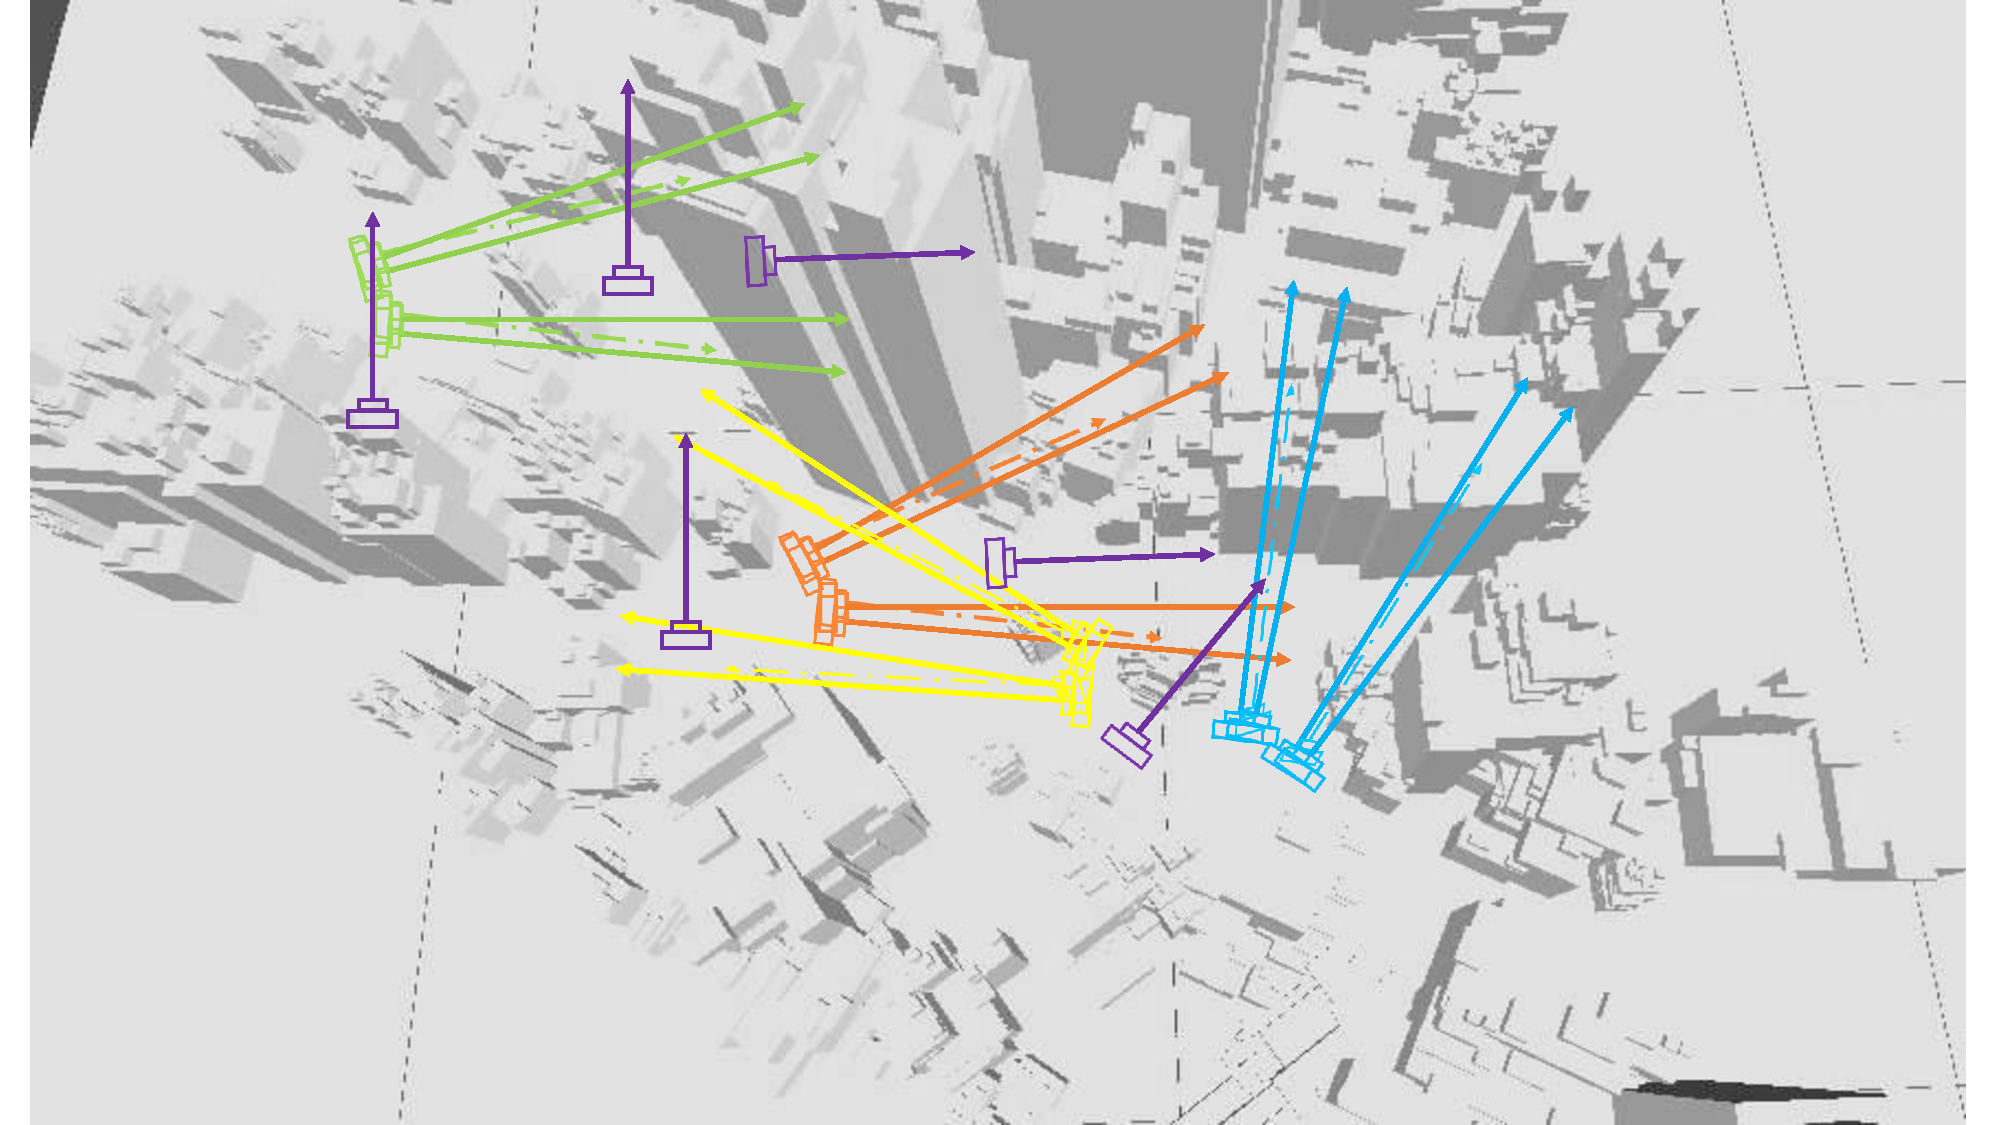
\includegraphics[width=0.9\columnwidth]{./fig/newCameraDeployment.pdf}
\caption{\label{fig::cameraDeployment}Camera deployment}
\end{subfigure}
\caption{\label{fig::cityAndCamera}City view and camera deployment}
\end{center}
\end{figure}

\ignore{
\begin{figure}
\begin{center}
\begin{subfigure}[b]{0.95\columnwidth}
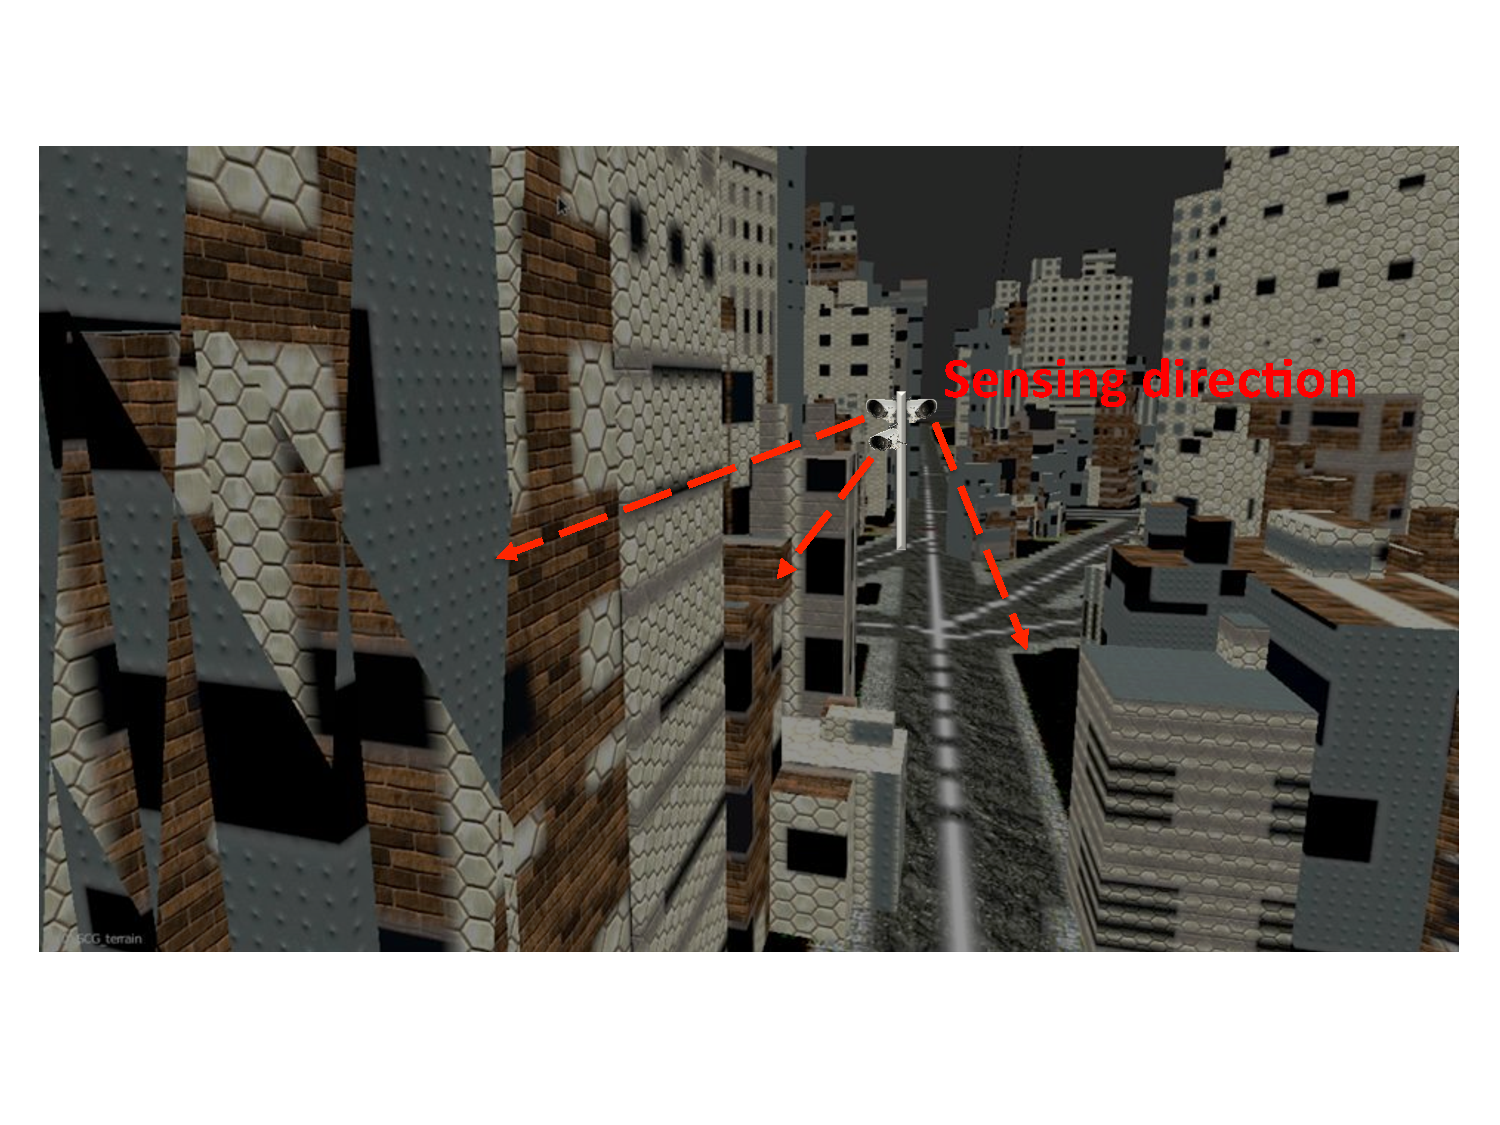
\includegraphics[width=0.95\columnwidth]{./fig/cameraAtCrossroad.pdf}
\caption{\label{fig::crossroadCamera}Camera deployment}
\end{subfigure}
\hfill
\begin{subfigure}[b]{0.95\columnwidth}
\includegraphics[width=0.95\columnwidth]{./fig/imageAtCrossroad.pdf}
\caption{\label{fig::testImages}Testing images}
\end{subfigure}
\caption{\label{fig::givenCrossroad}Camera deployment and collected images at a
given crossroad}
\end{center}
\end{figure}
}
%

\subsection{Dominating Set Problem Evaluation}
\label{sec::DSEvaluation}
\begin{figure}
\begin{center}
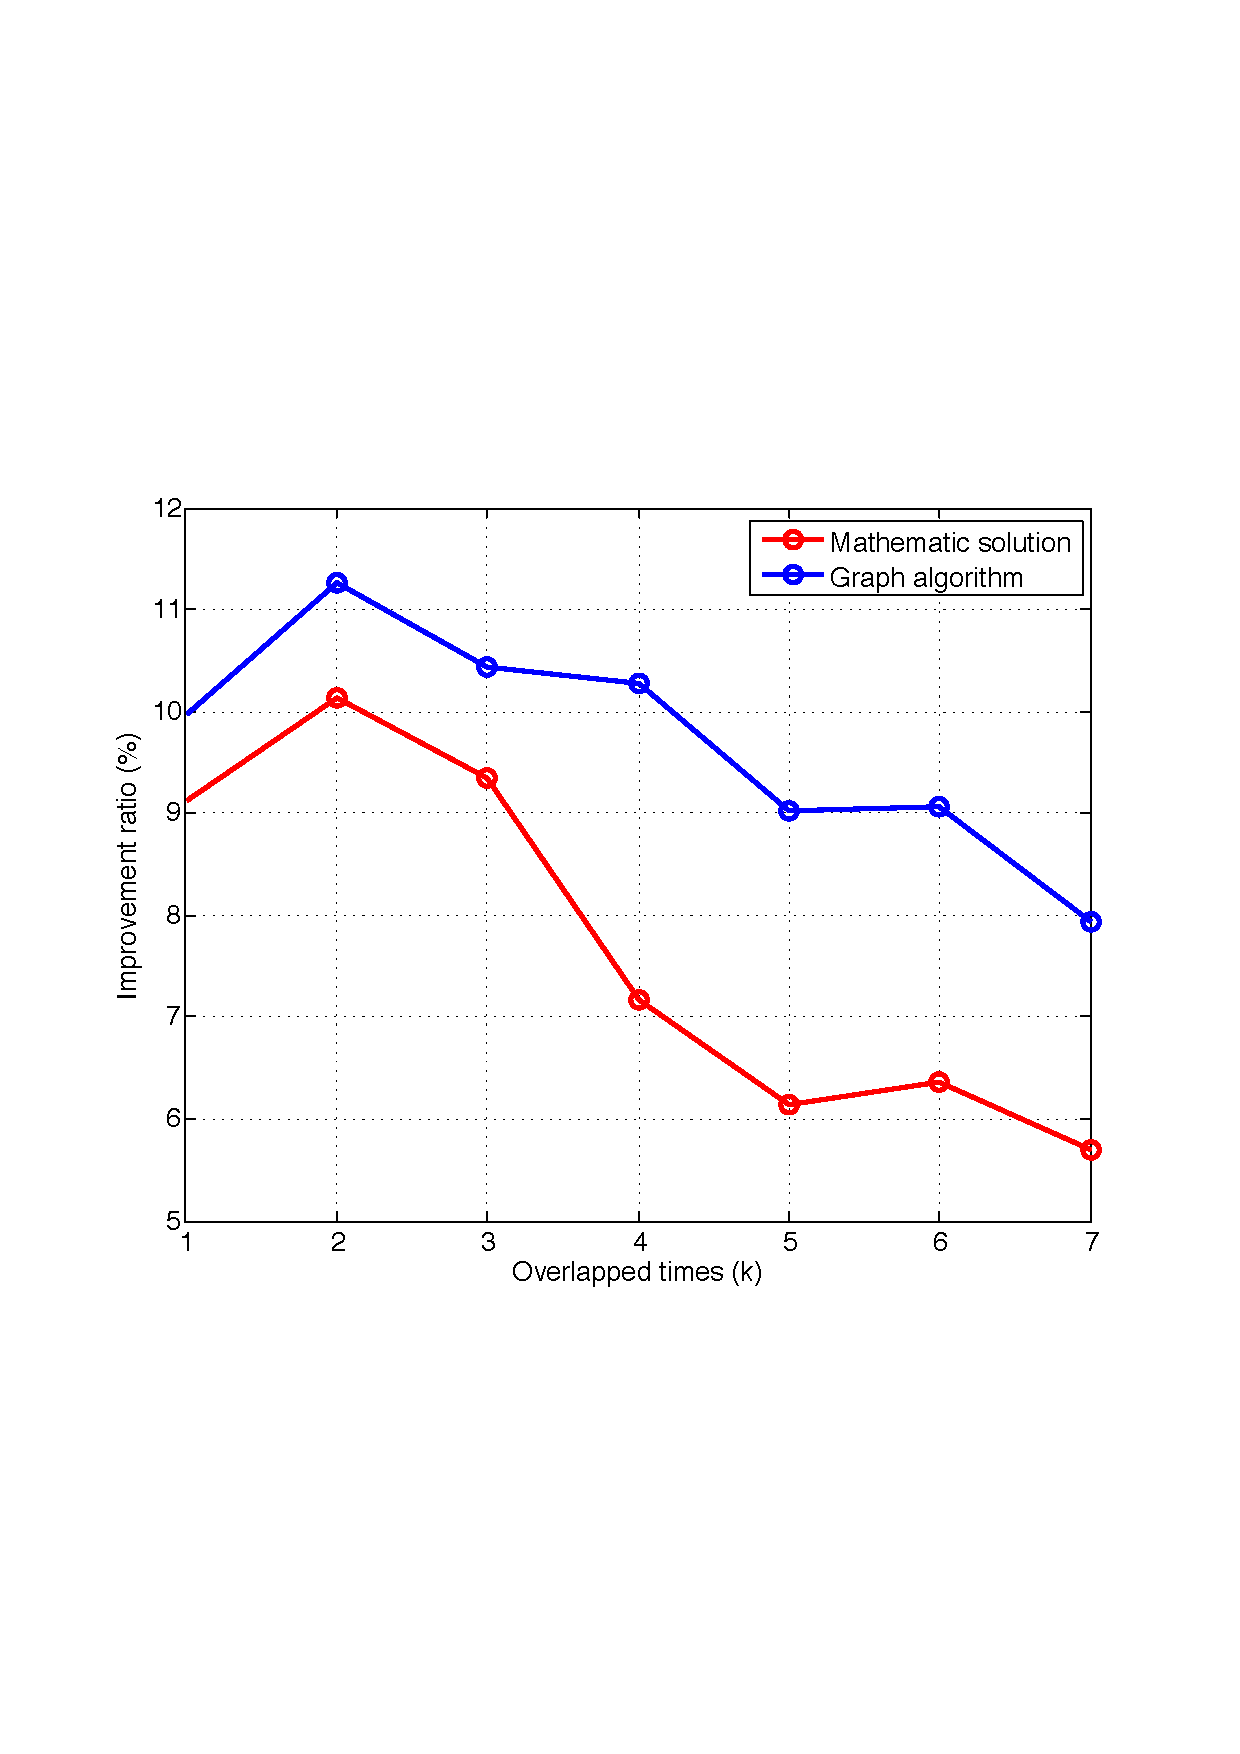
\includegraphics[width=0.9\columnwidth]{./fig/compareDSAlgorithm.pdf}
\caption{\label{fig::overlapped} Number of candidate reference broadcasters}
\end{center}
\end{figure}
{\color{blue}
As we mentioned before, changing the value of $k$ in
Problem~\eqref{eq::relaxedMDS} will cause a difference in the system
performance.
We here increase the value of $k$ from $1$ to $7$ and compare the mathematic
solution versus the heuristic graph algorithm.
The results is shown in Figure~\ref{fig::overlapped} and we can learn that
$k=2$ is the best choice in our network scenario.
This is because $k=2$ tends to select a proper amount of broadcasters for
independent transmission.
Therefore, if we increase the value of $k$ becomes larger than $2$, it happens
that there are too many independent transmitters and the advantage of
overhearing is not that evident.
However, we still want to argue that if the network becomes larger, increasing
the value $k$ is necessary to keep the overhearing performance.
}

\subsection{Experiment Results}
\label{sec:ExperimentResults}

\begin{figure}
\begin{center}
%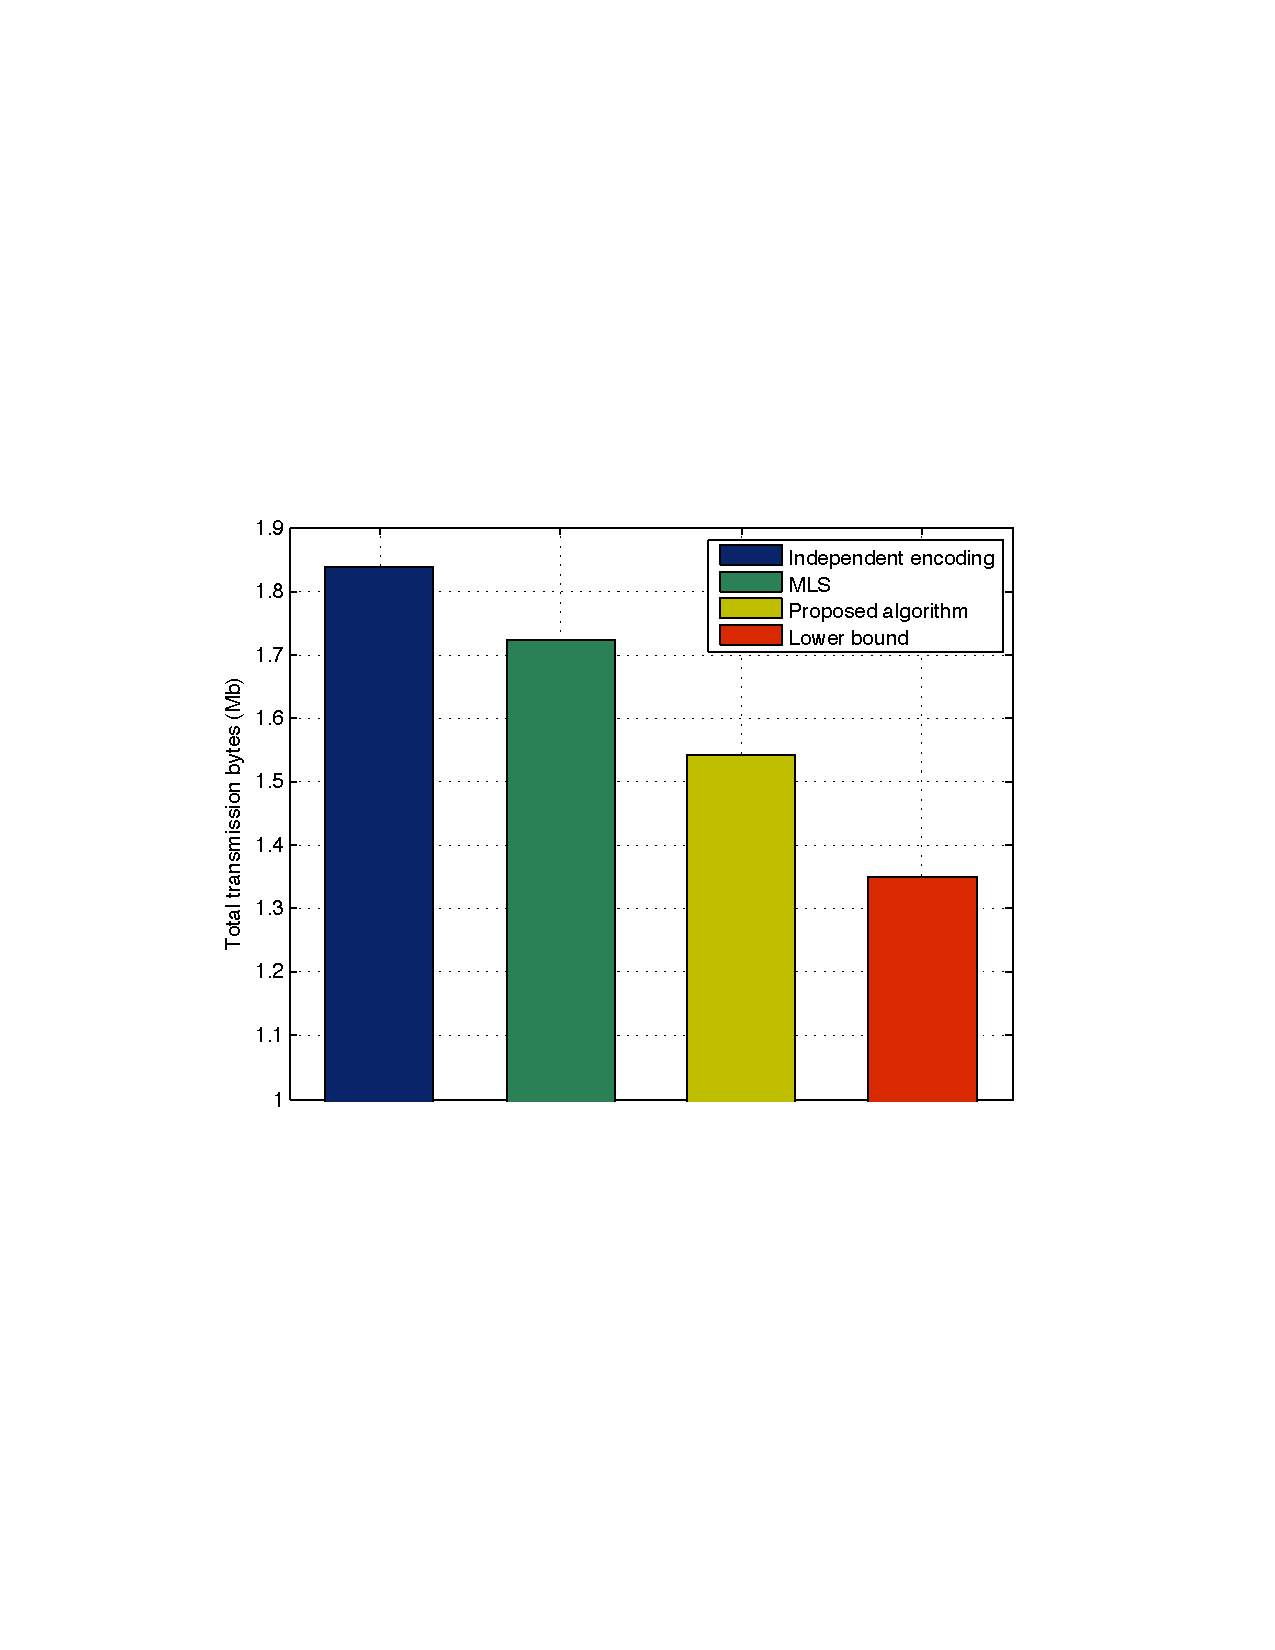
\includegraphics[width=0.95\columnwidth]{./fig/transByte.pdf}
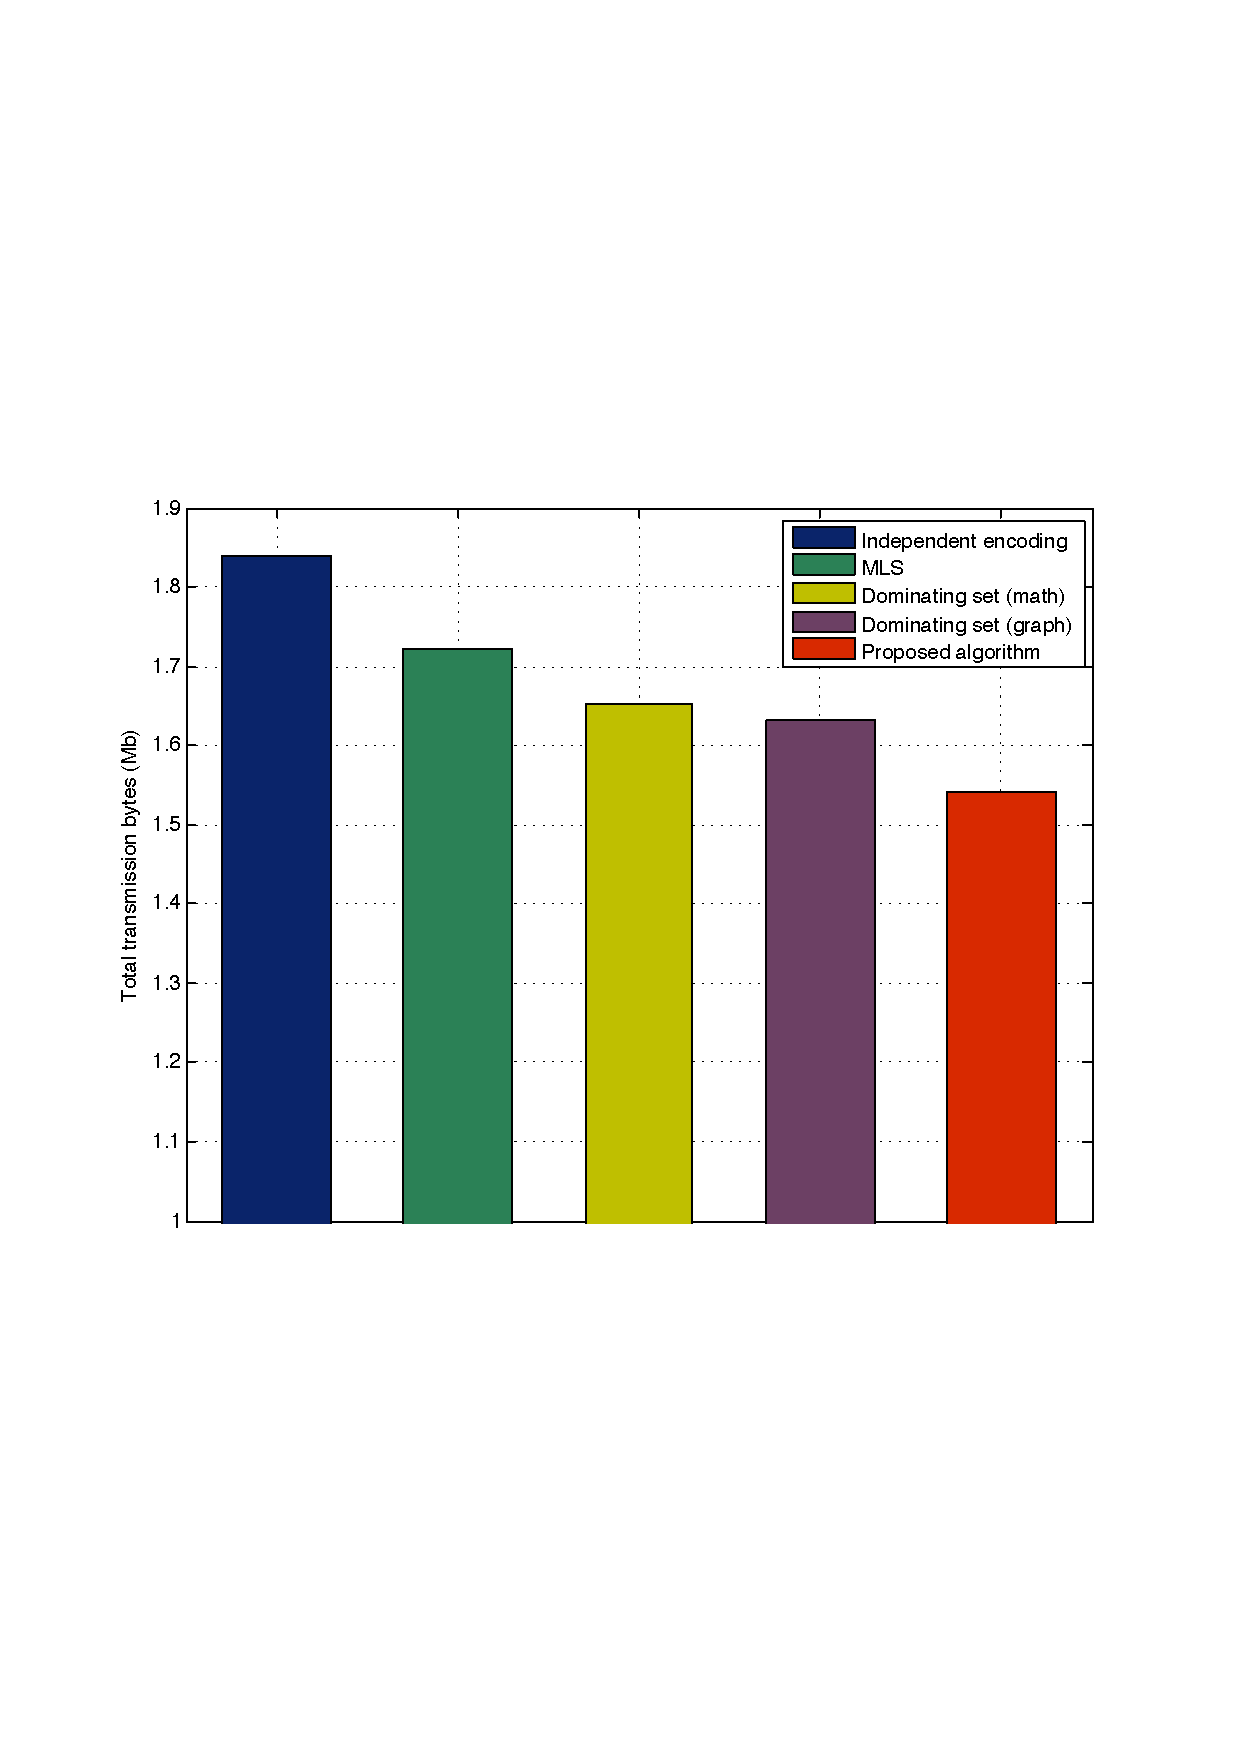
\includegraphics[width=0.9\columnwidth]{./fig/transByte5.pdf}
\caption{\label{fig::transByte}Performance comparison}
\end{center}
\end{figure}

%By using the experiment settings described in
%Section~\ref{sec::ExperimentSettings}, we show our experiment results about
%the total required encoded bits in this section under the image resolution of
%${1280 \times 720}$.
To evaluate the performance of the proposed algorithm, we compare against the
MLS algorithm proposed in~\cite{MLS}.
%the performance of our proposed algorithm with the MLS (maximum
%lifetime scheduling) problem, which has been well investigated in~\cite{MLS}.
The authors in~\cite{MLS} solve a {\em relaxed integer programming} problem to obtain
the probability that a camera should overhear transmissions of other cameras.
%of a camera should whether overhear others' transmission or
%transmit independently.
Since the binary decision for each camera is made by approximating the probability
thus solved,
%However, their approximation algorithm for transforming the obtained
%probability into an integer value seems too conservative.
there is performance loss during the transformation.
%That is, there might be too many cameras perform independent encoding, causing
%an inefficient usage of the limited radio resource.
%
Figure~\ref{fig::transByte} shows that MLS can improve the baseline performance
(all cameras perform independent encoding) for $6.3 \%$,
%shows that the improvement ratio of the MLS algorithm is about $6.3 \%$ while our
whereas {\color{blue} the dominating set problem has a $11.2 \%$ performance
gain for graph algorithm while the improvement of mathematic solution is
$10.1 \%$. Most important of all,} the proposed algorithm can achieve a
$16.2 \%$ improvement.
%
The result substantiates the benefits of the proposed scheduling algorithm and
motives further investigation along this direction.
%Therefore, we argue that there is a considerable performance gain between our
%proposed scheduling algorithm than the MLS algorithm proposed in~\cite{MLS}. 
%\section{Conclusion}
\label{sec:Conclusion}

\bibliographystyle{IEEEtran}
\bibliography{reference}

\end{document} 